\section{Experiments}

\subsection{Experimental Setup}
For the experiments with ResNet-18 on CIFAR-10 and DenseNet-121 on CIFAR-100, we use a single instance of P-100 GPU with 16GBs of memory.

We also use data from the UCR archive, with the main representative: 50 words time-series dataset with 270 values per data point, 50 classes, 450 train data points, 455 test data points, 2 MB in size. One of the best peforming CNN models for the data is a 3 layer Fully Convolutional Neural Network (FCN) with filter sizes: 8, 5, 3. The number of filter banks is: 128, 256, 128.~\footnote{http://bit.ly/2FbdQNV}. 
%We run the experiments on an on-premise server: GPU Pascal, GeForce GTX 1080 Ti, 3584 cores, max clock 1582 MHz, 10.6 single precision TFLOPS and 11GBs of main memory.

Our methodology is to measure the memory usage on GPU by counting the size of the allocated tensors. The direct measurement of hardware counters is imprecise because PyTorch uses a caching memory allocator to speed up memory allocations and incurs much higher memory usage than is actually needed at a given point in time.

\subsection{DenseNet-121 on CIFAR-100}
We train DenseNet-121 (with growth rate 12) on the CIFAR-100 dataset. 

\begin{figure}[t]
  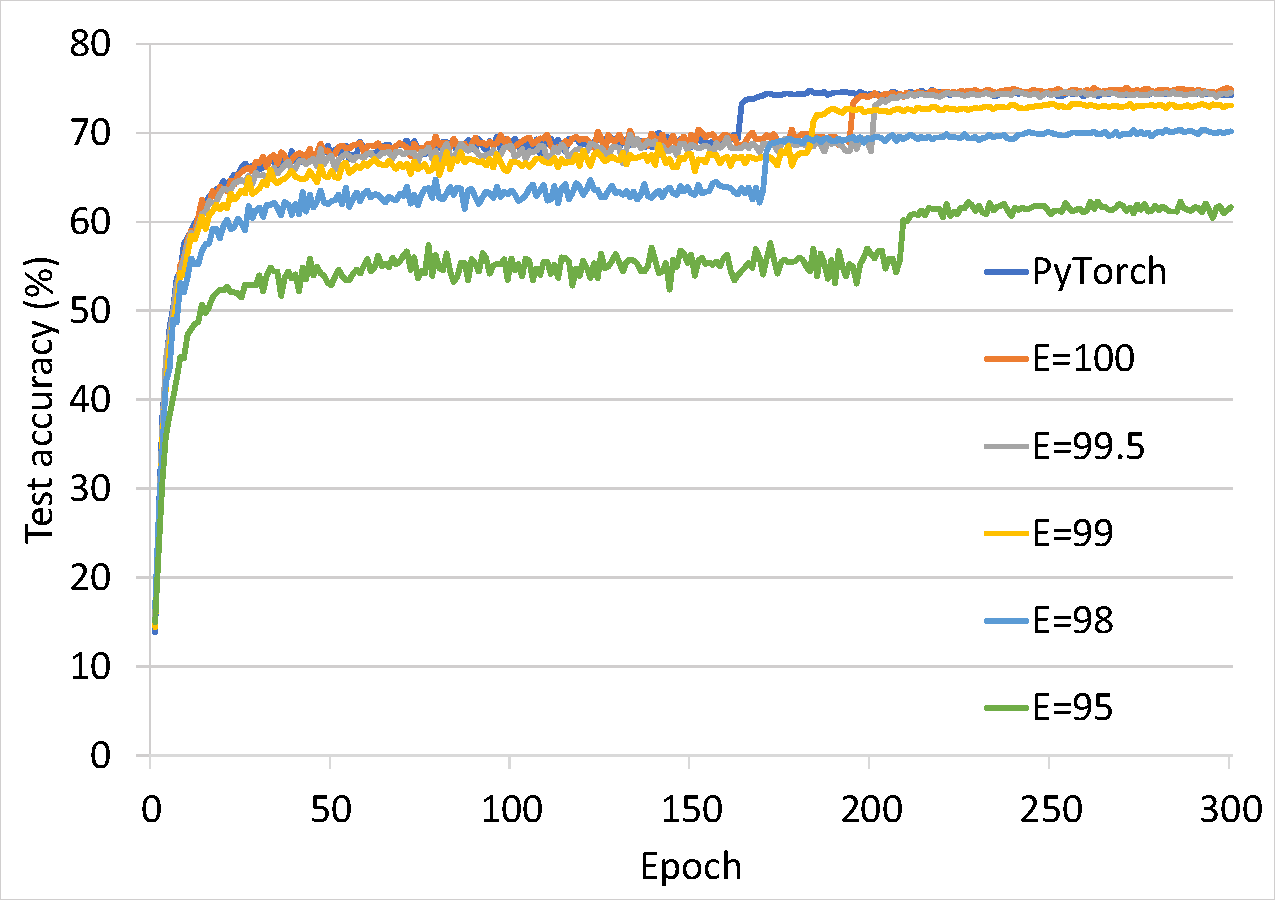
\includegraphics[width=0.95\linewidth]{DenseNet121CIFAR100TestAccuracy.pdf} %width=\linewidth]
  \caption{{\it Comparing test accuracy during training for CIFAR-100 dataset trained on DenseNet-121 (growth rate 12) architecture using convolution from PyTorch and FFT-based convolutions with different energy rates preserved.}}
  \label{fig:DenseNet121CIFAR100TestAccuracy}
\end{figure}

In Figure~\ref{fig:DenseNet121CIFAR100TestAccuracy} we show small differences in test accuracy during training between models with different levels of energy preserved for the FFT-based convolution.

\begin{figure}[t]
  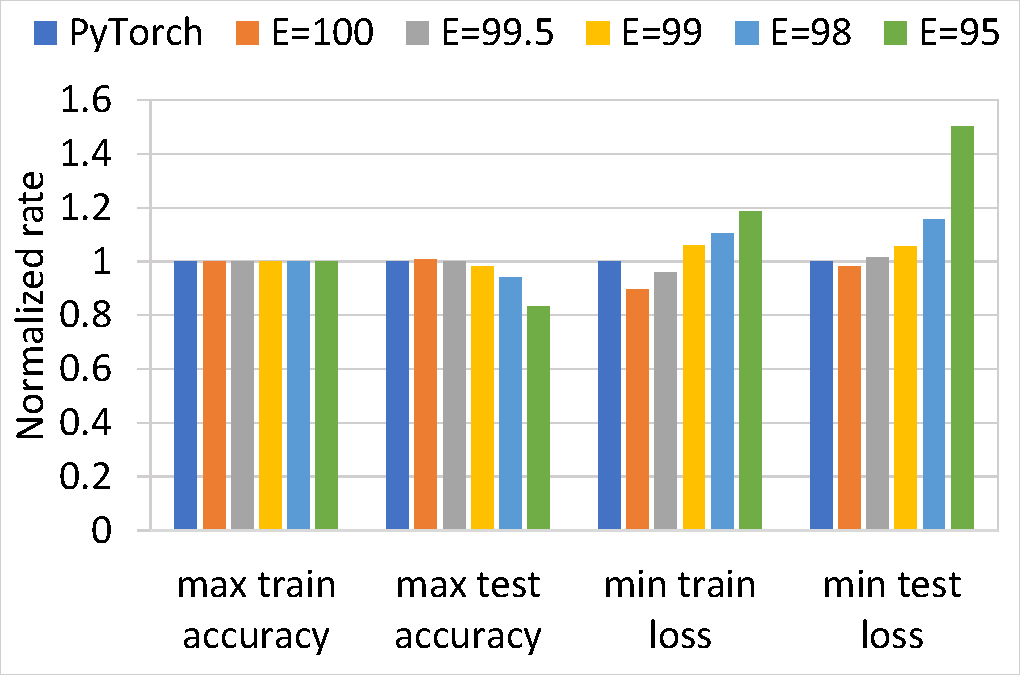
\includegraphics[width=0.95\linewidth]{DenseNet121CIFAR100NormalizedRateTestTrainAccuracyLoss.pdf} %width=\linewidth]
  \caption{{\it Comparing accuracy and loss for test and train sets from CIFAR-100 dataset trained on DenseNet-121 (growth rate 12) architecture using convolution from PyTorch and FFT-based convolutions with different energy rates preserved.}}
  \label{fig:DenseNet121CIFAR100NormalizedRateTestTrainAccuracyLoss}
\end{figure}

In Figure~\ref{fig:DenseNet121CIFAR100NormalizedRateTestTrainAccuracyLoss} we show small differences in accuracy and loss between models with different convolution implementations. The results were normalized with respect to the values obtained for the standard convolution used in PyTorch.  

\subsection{Reduced Precision and Bandlimited Training}
In Figure~\ref{fig:micro-mem}
 %and~\ref{fig:micro-gpu} 
 we plot the maximum allocation of the GPU memory during 3 first iterations. Each iteration consists of training (forward and backward passes) followed by testing (a single forward pass). We use CIFAR-10 data on ResNet-18 architecture. We show the memory profiles of RPA (Reduced Precision Arithmetic), bandlimited training, and applying both. A detailed convergence graph is shown in Figure~\ref{fig:fp16}.
 
 \begin{figure}[t]
  
\includegraphics[width=0.95\linewidth]{figures/fp16-fp32-fft50/fp32_fp16_fft50-2.pdf} %width=\linewidth]
  \caption{{\it Train and test accuracy during training for CIFAR-10 dataset trained on ResNet-18 architecture using convolution from PyTorch (fp32), mixed-precision (fp16) and FFT-based convolutions with 50\% of compression for intermediate results and filters (fft50). The highest test accuracy observed are: 93.69 (fp32), 91.53 (fp16),	92.32 (fft50).
}}
  \label{fig:fp16}
\end{figure}

\begin{figure}[t]
%   \includegraphics[width=0.95\linewidth]{figures/micro-analysis/no_mem_test_data_utilization_train_test_3_iterations/Memory-utilization.pdf}
  %\includegraphics[width=0.95\linewidth]{figures/micro-analysis/mem_test_mem_used_train_test_3_iterations/MemoryUsed-utilization.pdf}%width=\linewidth]
%   \includegraphics[width=0.95\linewidth]{figures/micro-analysis/mem_test_mem_used_train_test_3_iterations_only_main_fp16_correct_compress_rate/MemoryUsed-utilization.pdf}%width=\linewidth]
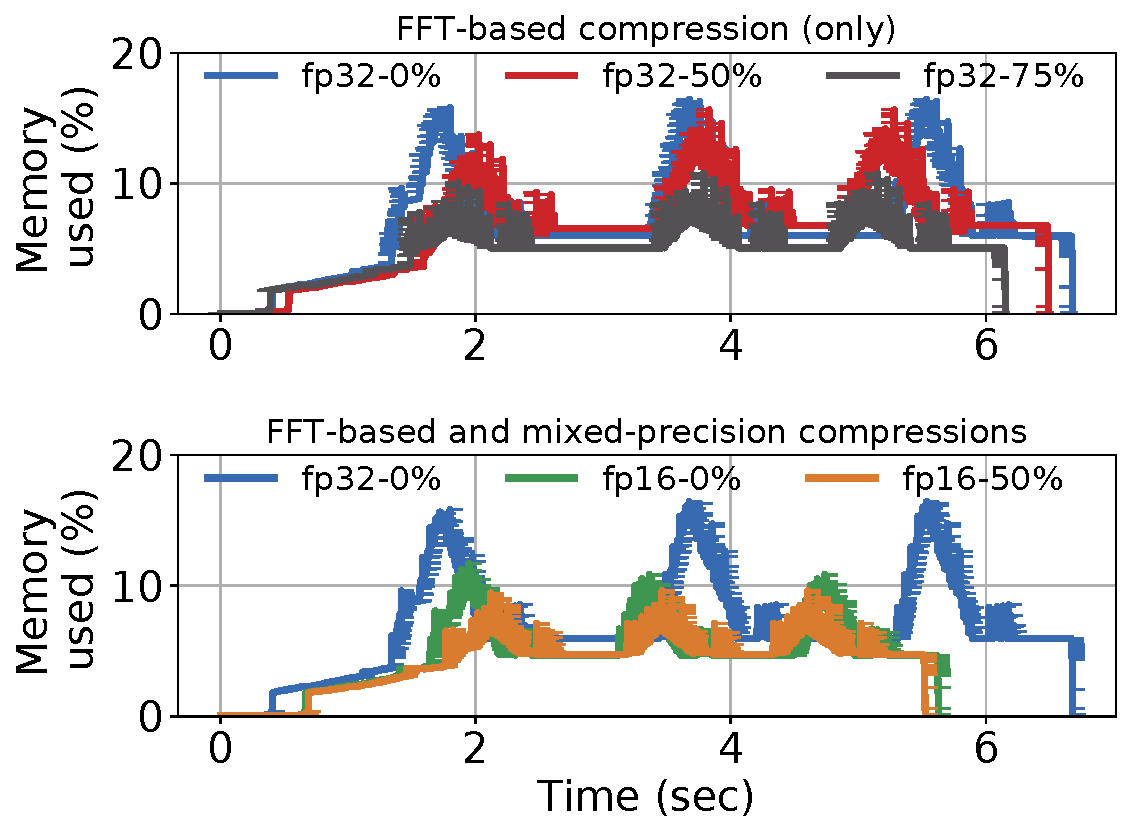
\includegraphics[width=0.95\linewidth]{MemoryUsed-utilization-font.pdf}
  \caption{{\it Memory used (\%)  for the first 3 iterations (train and test) with mixed-precision and FFT-based compression techniques. Mixed precision allows only a certain level of compression whereas with the FFT based compression we can adjust the required compression and accuracy. The two methods can be combined (fp16-50\%).
}}
  \label{fig:micro-mem}
\end{figure}

% \begin{figure}[t]
%   \includegraphics[width=0.95\linewidth]{figures/micro-analysis/GPU-utilization.pdf} %width=\linewidth]
%   \caption{{\it GPU utilization (\%) is lower with higher compression.
% }}
%   \label{fig:micro-gpu}
% \end{figure}

\subsection{Resource Usage vs Accuracy} 
The full changes in normalized resource usage (GPU memory or time for a single epoch) vs accuracy are plotted in Figure~\ref{fig:normalized_performance_sup}.

% FFT-ed tensors in PyTorch place the lowest frequency coefficients in the corners. For compression, we extract parts of a tensor from its top-left and bottom-left corners, then concatenate them. For the decompression part, we fill in the discarded parts with zeros. These operations have a non-negligible cost. The overhead might be minimized in 2D case if the DC component would be moved to the center and the compression would only extract the middle coefficients (by slicing and without a need to stitch together different parts of a tensor) so that the compressed tensor would remain contiguous.

% DenseNet-121 shows a significant drop in GPU memory usage with relatively low drop in accuracy. On the other hand, ResNet-18 is a smaller network and after about 50\% of the compression ratio, other than convolutional layers start dominate the memory usage. The convolution operation remains the major computation bottleneck and we decrease it with higher compression.

% For ResNet-50 on ImageNet, we observe a substantial drop in memory usage after applying our compression and similar behavior in terms of the time per epoch to the ResNet-18 model on CIFAR-10.

\begin{figure}[t]
    %   
\includegraphics[width=0.95\linewidth]{figures/gpu_time_mem_alloc_accuracy/gpu_time_mem_alloc_accuracy.pdf} %width=\linewidth]
    % width=0.95
    % 
\includegraphics[width=0.95\linewidth]{figures/gpu_time_mem_alloc_accuracy/gpu_time_mem_alloc_accuracy.pdf} %width=\linewidth]
    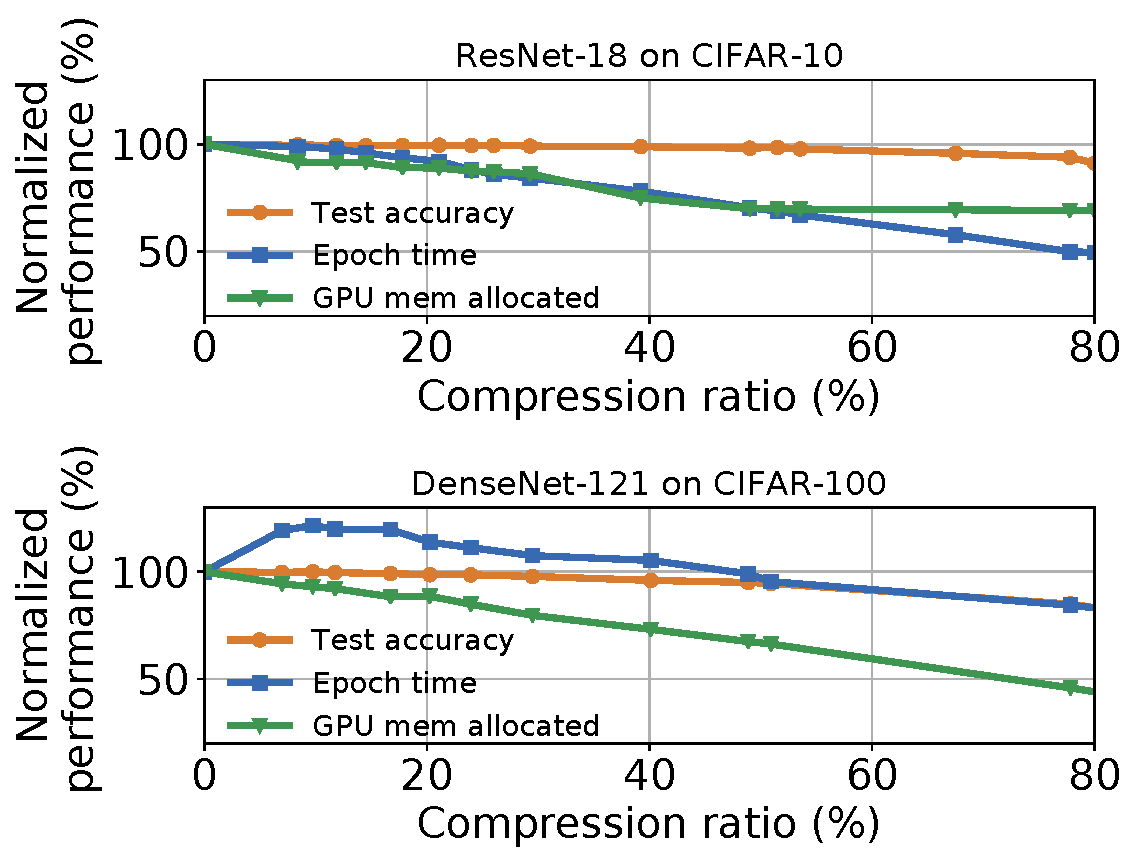
\includegraphics[width=0.95\linewidth]{gpu_time_mem_alloc_accuracy_font.pdf}
    \caption{{\it Normalized performance (\%) between models trained with different FFT-compression ratios.}}
    \label{fig:normalized_performance_sup}
\end{figure}

\subsection{Dynamic Changes of Compression}

Deep neural networks can better learn the model if the compression is fixed and does not change with each iteration depending on the distribution of the energy within the frequency coefficients of a signal. %However, the dynamic compression based on the energy preserved shows that at the beginning of the training the network is focused on the low frequency coefficients and as the training unfolds, more and more coefficients are taken into account. The compression based on preserved energy does not steadily converge to a certain compression ratio but can decrease significantly and abruptly even at the end of the training process (especially, for the initial layers). 

We observe that the compression can be applied more effectively to the first layers and the deeper the layers the less compression can be applied (for a given energy level preserved).

The dynamic and static compression methods can be combined. We determine how much compression should be applied to each layer via the energy level required to be saved in each layer and use the result to set the static compression for the full training.  
The sparsification in the Winograd domain requires us to train a full (uncompressed) model, then inspect the Winograd coefficients of the filters and input maps and zero-out these of them which are the smallest with respect to their absolute values, and finally retrain the compressed model. In our approach, we can find the required number of coefficients to be discarded with a few forward passes (instead of training the full network), which can save time and also enables us to utilize less GPU memory from the very beginning with the dynamic compression. 

\subsection{Compression Based on Preserved Energy}
%\TODO{Our goal is to provide similar experiments to the ones presented in~\cite{liu2018efficient}.xs}

%The first step was to implement the forward and backward passes for the 2D convolution with compression in the FFT domain. 
%Then, we have to create the VGG-nagadomi network~\cite{nagadomi} in PyTorch or leverage the latest models from~\cite{kuangliu}. The minor issue is that none of the network architecture uses filters of sizes bigger than 3x3.
There are a few ways to compress signals in the frequency domain for 2D data. The version of the output in the frequency domain can be compressed by setting the DC component in the top left corner in the frequency representation of an image or a filter (with the absolute values of coefficients decreasing towards the center from all its corners) and then slicing off rows and columns. The heat maps of such a representation containing the absolute value of the coefficients is shown in Figure~\ref{fig:fft_heat_map}.

\begin{figure}[t]
\centering
  %
\includegraphics[width=\linewidth]{figures/conv2D-cifar10-leNet-test-accuracy.pdf} %width=\linewidth]
  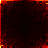
\includegraphics[scale=6.0]{xfft_abs.pdf} %width=\linewidth]
  %
\includegraphics[scale=5.0]{figures/heat-maps/xfft_abs.pdf}
  \caption{{\it A heat map of absolute values (magnitudes) of FFT coefficients with linear interpolation and the max value colored with white and the min value colored with black. The FFT-ed input is a single (0-th) channel of a randomly selected image from the CIFAR-10 dataset.}}
  \label{fig:fft_heat_map}
\end{figure}

The number of preserved elements even for 99\% of the preserved energy is usually small (from 2X to 4X smaller than the initial input). Thus, for the energy based compression, we usually proceed starting from the DC component and then adding rows and columns in the vertically mirrored \textit{L} fashion. It can be done coarse-grained, where we just take into account the energy of the new part of row or column to be added, or fine-grained, where we add elements one by one and if not the whole row or column is needed, we zero-out the remaining elements of both an activation map and a filter.

\subsection{Visualization of the Compression in 1D}
We present the visualization of our FFT-based compression method in~\ref{fig:fft_compresion_1D}. The magnitude is conveniently plotted in a logarithmic scale (dB).

\begin{figure}[t]
\centering
  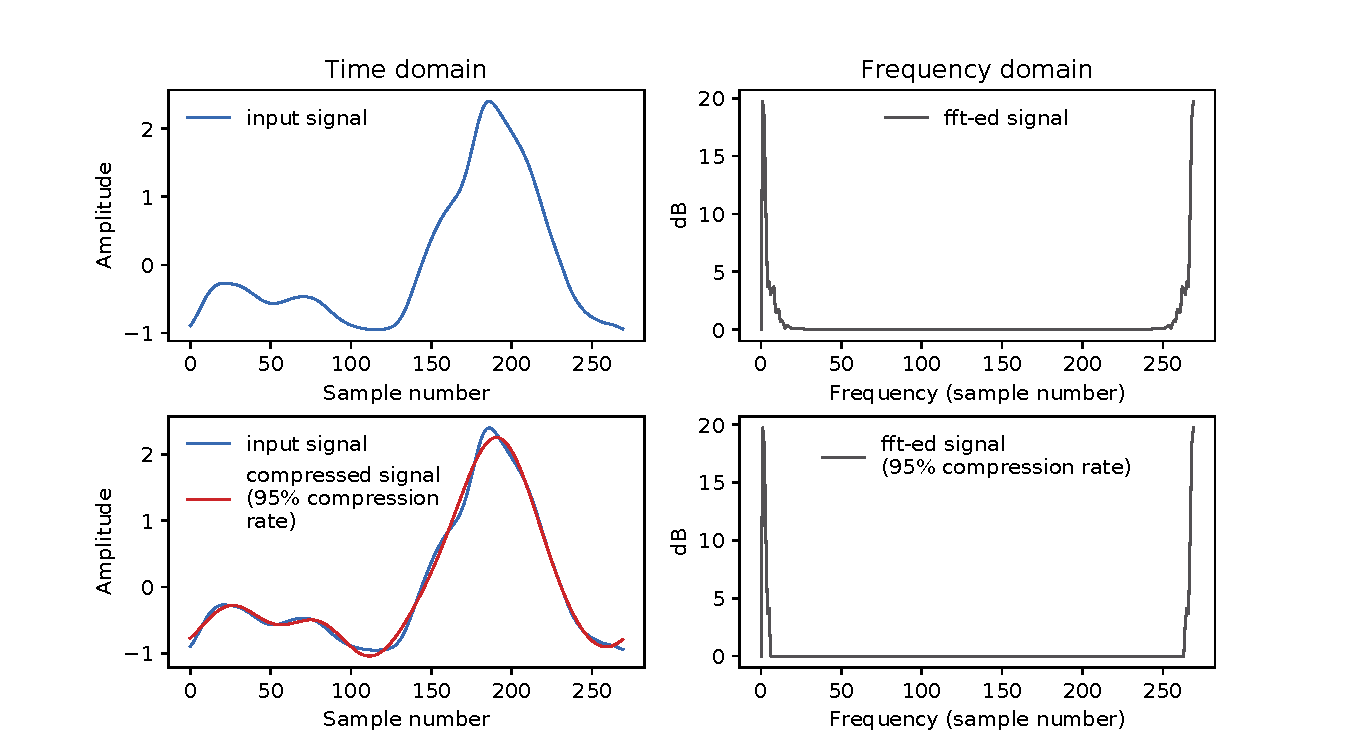
\includegraphics[scale=0.4]{original-1D-2.pdf} %width=\linewidth]
  %
\includegraphics[scale=5.0]{figures/heat-maps/xfft_abs.pdf}
  \caption{{\it We present a time series (signal) from the UCR archive and fifty words dataset in the top-left quadrant. Its frequency representation (as power spectrum) after normalized FFT transformation is shown in the top-right quadrant. The signal is compressed by 95\% (we zero out the \textit{middle} Fourier coefficients) and presented in the bottom-right quadrant. We compare the initial signal and its compressed version in the bottom-left quadrant. The magnitudes of Fourier coefficients are presented in the logarithmic (dB) scale.}}
  \label{fig:fft_compresion_1D}
\end{figure}


% \begin{figure}[t]
% \centering
%   %
\includegraphics[width=\linewidth]{figures/conv2D-cifar10-leNet-test-accuracy.pdf} %width=\linewidth]
%   \includegraphics[width=\columnwidth]{figures/visualizations/visualize-fft.png} %width=\linewidth]
%   %
\includegraphics[scale=5.0]{figures/heat-maps/xfft_abs.pdf}
%   \caption{{\it We present an original image from the ImageNet dataset with label: \textit{bull mastiff} in the first row and the 50\% compressed Fourier domain in the second row. The heat maps of magnitudes of Fourier coefficients are presented in a logarithmic scale (dB) with linear interpolation and the max value is colored with white while the min value is colored with black. The frequency representation is plotted for a single (0-th) channel.}}
%   \label{fig:fft_compresion}
% \end{figure}

\subsection{Energy Based Compression for ResNet-18}
Figure~\ref{fig:linearCorrelationAccuracyEnergyPreserved} shows the linear correlation between the accuracy of a model and the energy that was preserved in the model during training and testing. Each point in the graph requires a fool training of a model for the indicated energy level preserved. 
\begin{figure}[t]
  %
\includegraphics[width=\linewidth]{figures/conv2D-cifar10-leNet-test-accuracy.pdf} %width=\linewidth]
  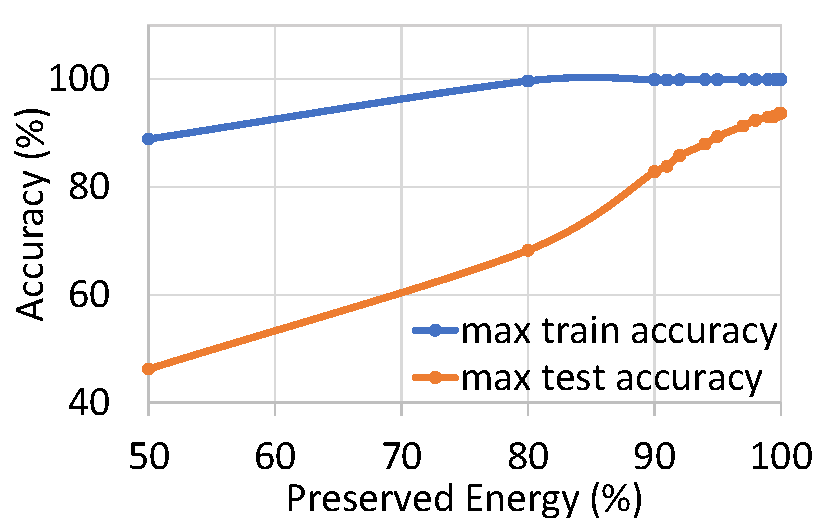
\includegraphics[width=\linewidth]{Cifar10ResNet18EnergyAccuracyDependence3.pdf} %width=\linewidth]
  \caption{{\it The linear correlation between the accuracy of a model and the energy that was preserved in the model during training and testing.}}
  \label{fig:linearCorrelationAccuracyEnergyPreserved}
\end{figure}

Figure~\ref{fig:Cifar10ResNet18TestAccuracyPreservedEnergy} shows the test accuracy during the training process of the ResNet-18 model on the CIFAR-10 dataset. 
\begin{figure}[t]
  %
\includegraphics[width=\linewidth]{figures/conv2D-cifar10-leNet-test-accuracy.pdf} %width=\linewidth]
  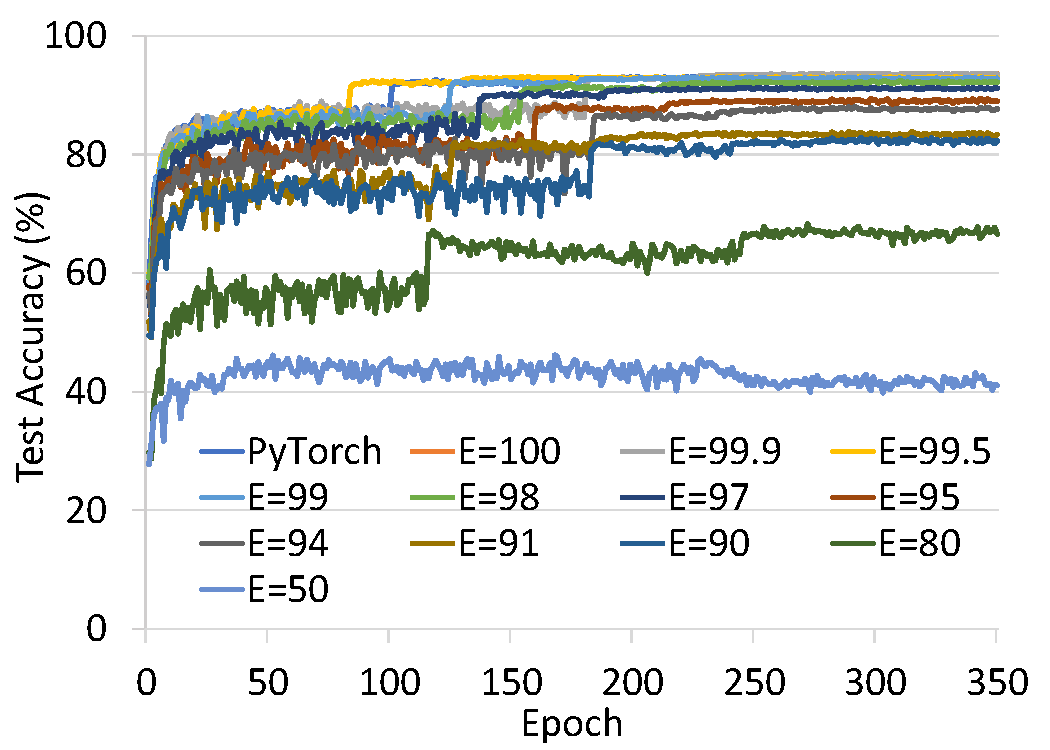
\includegraphics[width=\linewidth]{Cifar10ResNet18TestAccuracyPreservedEnergy.pdf} %width=\linewidth]
  \caption{{\it The test accuracy during the training process of the ResNet-18 model on the CIFAR-10 dataset.}}
  \label{fig:Cifar10ResNet18TestAccuracyPreservedEnergy}
\end{figure}

Figure~\ref{fig:Cifar10ResNet18TrainAccuracyPreservedEnergy} shows the train accuracy during the training process of the ResNet-18 model on the CIFAR-10 dataset. 
\begin{figure}[t]
  %
\includegraphics[width=\linewidth]{figures/conv2D-cifar10-leNet-test-accuracy.pdf} %width=\linewidth]
  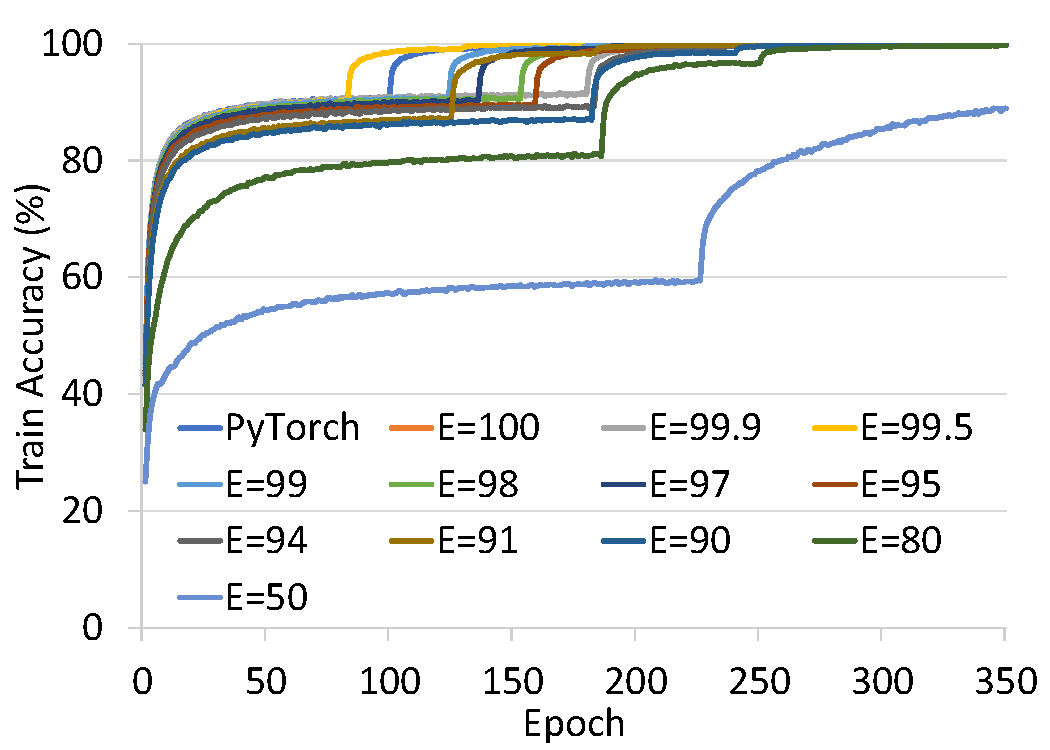
\includegraphics[width=\linewidth]{Cifar10ResNet18TrainAccuracyPreservedEnergy.pdf} %width=\linewidth]
  \caption{{\it The train accuracy during the training process of the ResNet-18 model on the CIFAR-10 dataset.}}
  \label{fig:Cifar10ResNet18TrainAccuracyPreservedEnergy}
\end{figure}

\begin{figure}[t]
  %
\includegraphics[width=\linewidth]{figures/conv2D-cifar10-leNet-test-accuracy.pdf} %width=\linewidth]
  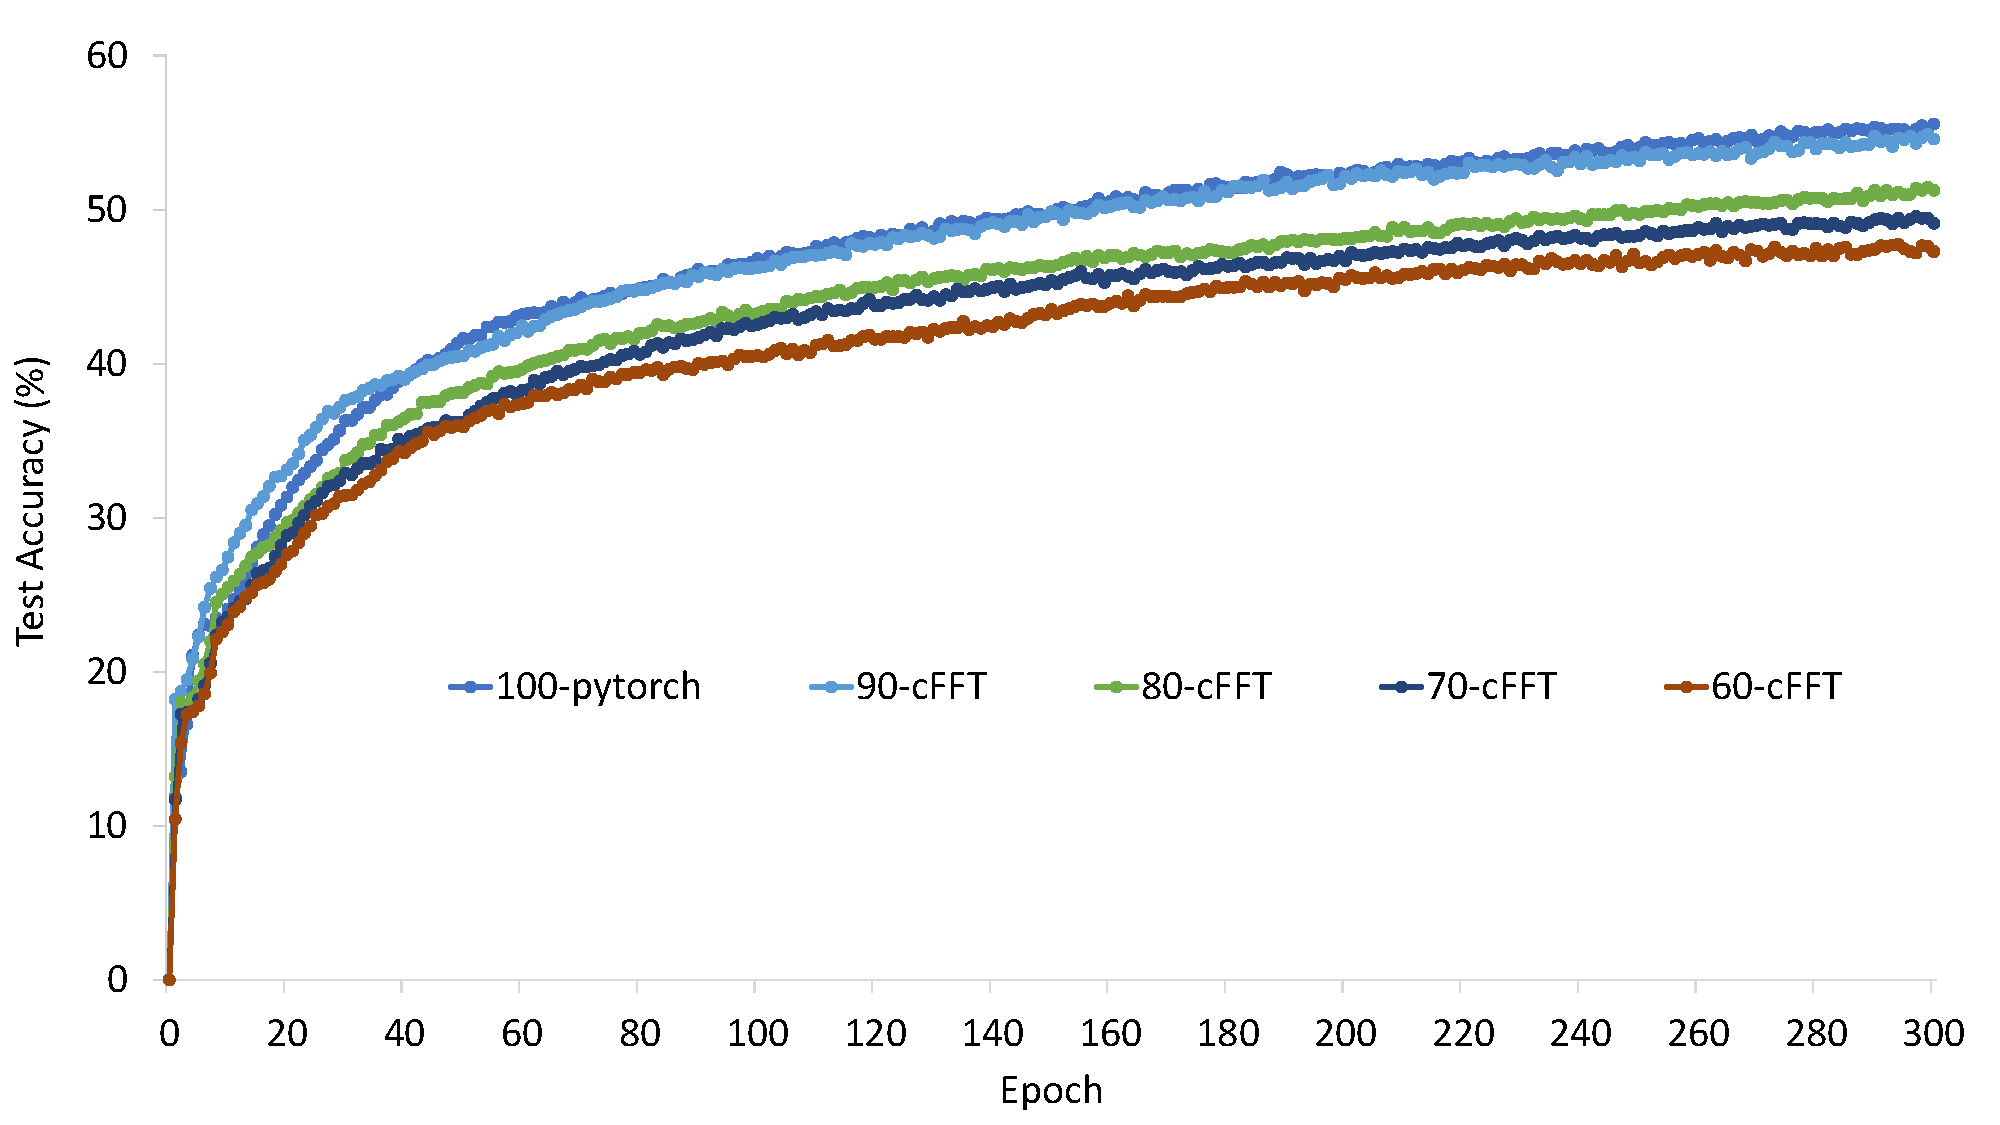
\includegraphics[width=\linewidth]{conv2D-cifar10-leNet-test-accuracy-only-every-10.pdf} %width=\linewidth]
  \caption{{\it A comparison of 2D convolution operation implemented in PyTorch and FFT version for different percentage of preserved energy (on the level of a batch).}}
  \label{fig:compareFFT2Dconv}
\end{figure}

\begin{figure}[t]
  %
\includegraphics[width=\linewidth]{figures/conv2D-cifar10-leNet-test-accuracy.pdf} %width=\linewidth]
  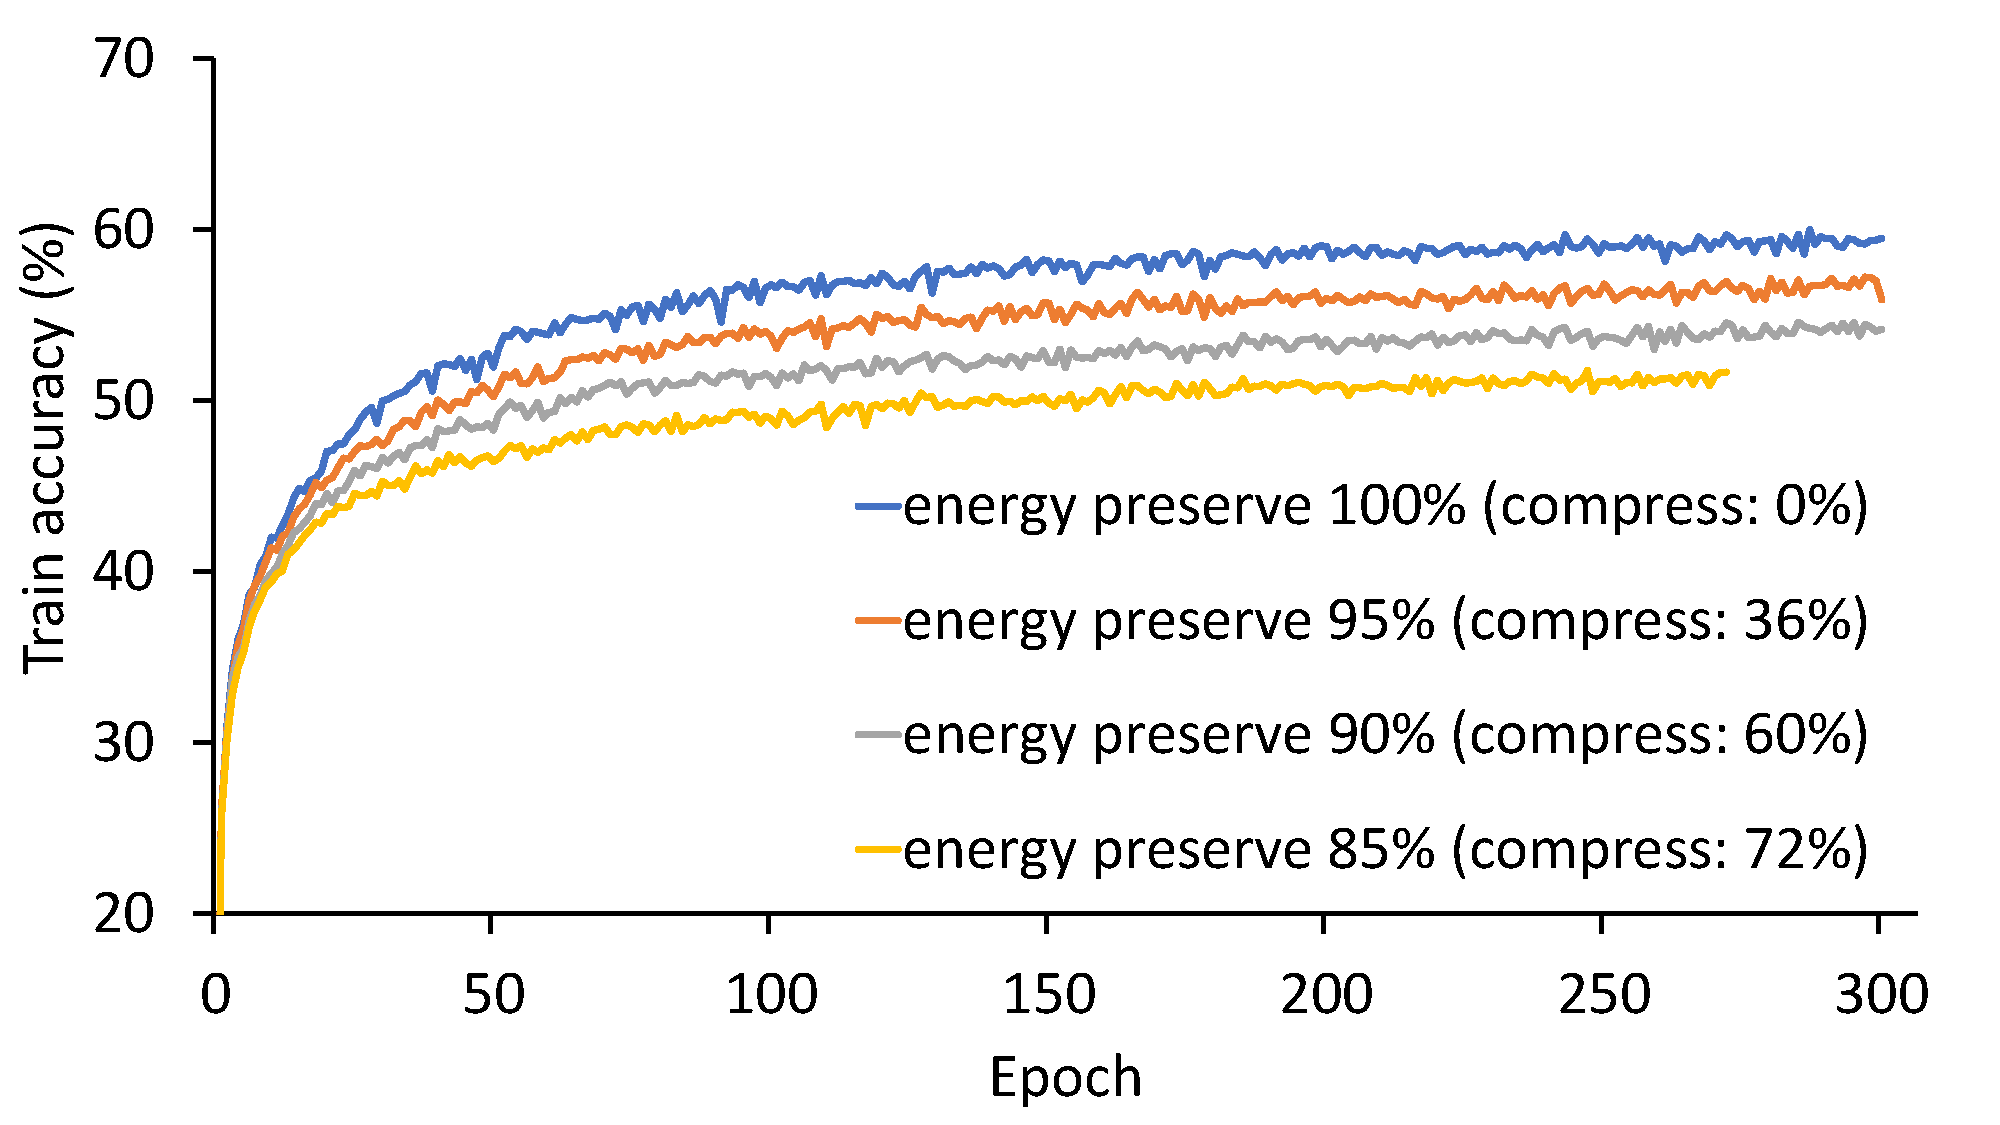
\includegraphics[width=\linewidth]{TrainAccuracyConv2DLeNet.pdf} %width=\linewidth]
  \caption{{\it Train accuracy for CIFAR-10 dataset on LeNet (2 conv layers) architecture
Momentum 0.9, batch size 64, learning rate 0.001  
.}}
  \label{fig:compareFFT2DconvTrainAccuracy}
\end{figure}

\begin{figure}[t]
  %
\includegraphics[width=\linewidth]{figures/conv2D-cifar10-leNet-test-accuracy.pdf} %width=\linewidth]
  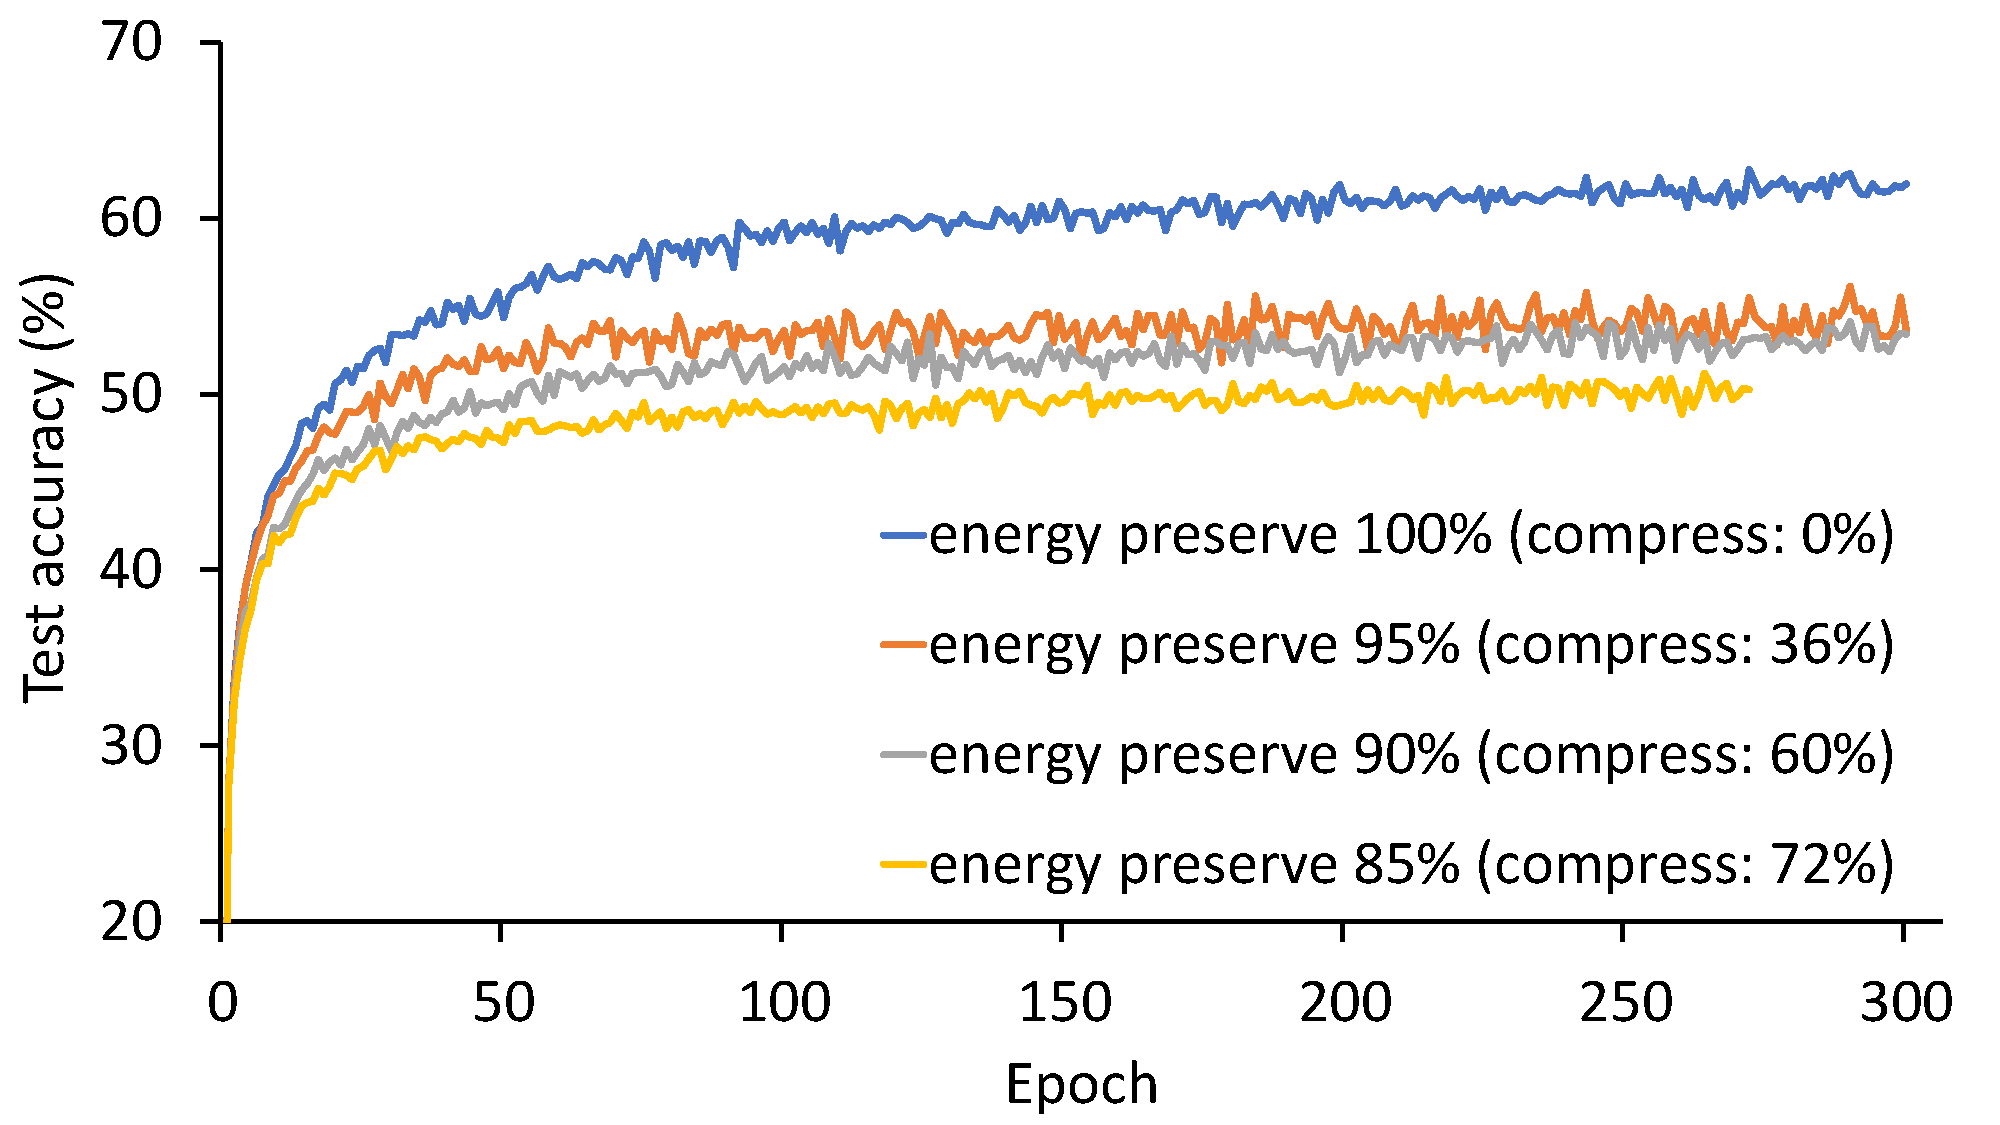
\includegraphics[width=\linewidth]{TestAccuracyConv2DLeNet.pdf} %width=\linewidth]
  \caption{{\it Test accuracy for CIFAR-10 dataset on LeNet architecture (2 conv layers, momentum 0.9, batch size 64, learning rate 0.001.}}
  \label{fig:compareFFT2DconvTestAccuracy}
\end{figure}

\subsection{Training vs. Inference Bandlimiting}
% \textbf{**? Please replace with 2D results**}
To further corroborate our points, consider a scheme where we train the network with one compression ratio and test with another (Figure~\ref{fig:compressionLeveslTrainTest}).

\begin{figure} \centering 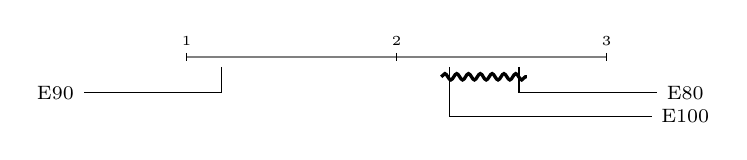
\begin{tikzpicture}[xscale=2]
%\node (Label) at  (01.9733,0.7) {\tiny{CD}}; % the label
%\draw[decorate,decoration={snake,amplitude=.4mm,segment length=1.5mm,post length=0mm}, very thick, color = black](01.3333, 0.5) -- (02.6133, 0.5);
%\foreach \x in {01.3333,02.6133} \draw[thick,color = black] (\x, 0.4) -- (\x, 0.6);
\draw[gray, thick](01.3333, 0) -- (04.0000, 0);
\foreach \x in {01.3333,02.6667,04.0000}\draw (\x cm,1.5pt) -- (\x cm, -1.5pt);
\node (Label) at (01.3333,0.2) {\tiny{1}};
\node (Label) at (02.6667,0.2) {\tiny{2}};
\node (Label) at (04.0000,0.2) {\tiny{3}};
\draw[decorate,decoration={snake,amplitude=.4mm,segment length=1.5mm,post length=0mm}, very thick, color = black](02.9500,-00.2500) -- ( 03.4940,-00.2500);
\node (Point) at (01.5560, 0){};  \node (Label) at (0.5,-00.4500){\scriptsize{E90}}; \draw (Point) |- (Label);
\node (Point) at (03.4440, 0){};  \node (Label) at (4.5,-00.4500){\scriptsize{E80}}; \draw (Point) |- (Label);
\node (Point) at (03.0000, 0){};  \node (Label) at (4.5,-00.7500){\scriptsize{E100}}; \draw (Point) |- (Label);
\end{tikzpicture}
\caption{Ranking of different compression ratios (80\%, 90\%, and 100\% energy preserved) during inference with model trained using no compression (90\% of energy preserved)}
\label{friedman1}
\end{figure}

\begin{figure} \centering 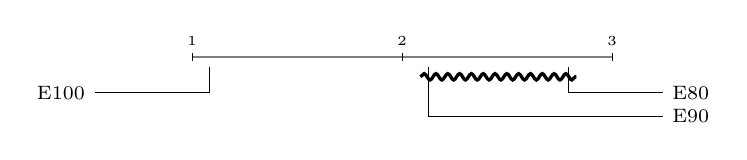
\begin{tikzpicture}[xscale=2]
%\node (Label) at  (01.9733,0.7) {\tiny{CD}}; % the label
%\draw[decorate,decoration={snake,amplitude=.4mm,segment length=1.5mm,post length=0mm}, very thick, color = black](01.3333, 0.5) -- (02.6133, 0.5);
%\foreach \x in {01.3333,02.6133} \draw[thick,color = black] (\x, 0.4) -- (\x, 0.6);
\draw[gray, thick](01.3333, 0) -- (04.0000, 0);
\foreach \x in {01.3333,02.6667,04.0000}\draw (\x cm,1.5pt) -- (\x cm, -1.5pt);
\node (Label) at (01.3333,0.2) {\tiny{1}};
\node (Label) at (02.6667,0.2) {\tiny{2}};
\node (Label) at (04.0000,0.2) {\tiny{3}};
\draw[decorate,decoration={snake,amplitude=.4mm,segment length=1.5mm,post length=0mm}, very thick, color = black](02.7833,-00.2500) -- ( 03.7727,-00.2500);
\node (Point) at (01.4440, 0){};  \node (Label) at (0.5,-00.4500){\scriptsize{E100}}; \draw (Point) |- (Label);
\node (Point) at (03.7227, 0){};  \node (Label) at (4.5,-00.4500){\scriptsize{E80}}; \draw (Point) |- (Label);
\node (Point) at (02.8333, 0){};  \node (Label) at (4.5,-00.7500){\scriptsize{E90}}; \draw (Point) |- (Label);
\end{tikzpicture}
\caption{Ranking of different compression ratios (80\%, 90\%, and 100\% energy preserved) during inference with model trained using no compression (100\% of energy preserved)}
\label{friedman2}
\end{figure}

We observe that the network is most accurate when the compression used for training is the same that is used during testing. We used the Friedman statistical test followed by the post-hoc Nemenyi test to assess the performance of multiple compression ratios during inference over multiple datasets. Figure~\ref{friedman1} shows the average rank of the test accuracies of different compression ratios during inference across 25 randomly chosen time-series data from the UCR Archive. The training was done while preserving 90\% of the energy. Inference with the same compression ratio (90\%) is ranked first, meaning that it performed the best in the majority of the datasets. The Friedman test rejects the null hypothesis that all measures behave similarly, and, hence, we proceed with a post-hoc Nemenyi test, to evaluate the significance of the differences in the ranks. The wiggly line in the figure connects all approaches that do not perform statistically differently according to the Nemenyi test. We had similar findings when training was done using no compression but compression was later applied during inference (see Figure~\ref{friedman2}). In other words, the network \emph{learns how to best leverage a band-limited operation to make its predictions}.
 
 Even so its performance degrades gracefully for tests with the compression level further from the one used during training. 
 In our opinions, the smooth degradation in performance is a valuable property of band-limiting. An outer optimization loop can tune this parameter without worrying about training or testing instability.

\subsection{Error Incurred by 2D Convolution with Compression}
We tried to measure how accurate the computation of the convolution result is when the compression is applied. An image from CIFAR-10 dataset (3x32x32) was selected and an initial version of a single filter (3x5x5, Glorot initialization). We did convolution using PyTorch, executed our convolution with compression for different compression ratios, and compared the results. The compression was measured relatively to the execution of our FFT-based convolution without any compression (100\% of the energy of the input image is preserved). The results show that for 2D convolution the relative error is already high (about 22.07\%) for a single index discarded (the smallest possible compression of about 6\%). However, after the initial abrupt change we observe a linear dependence between compression ratio and relative error until more than about 95\% of compression ratio, after which we observe a fast degradation of the result.

\begin{figure}[t]
  %
\includegraphics[width=\linewidth]{figures/conv2D-cifar10-leNet-test-accuracy.pdf} %width=\linewidth]
  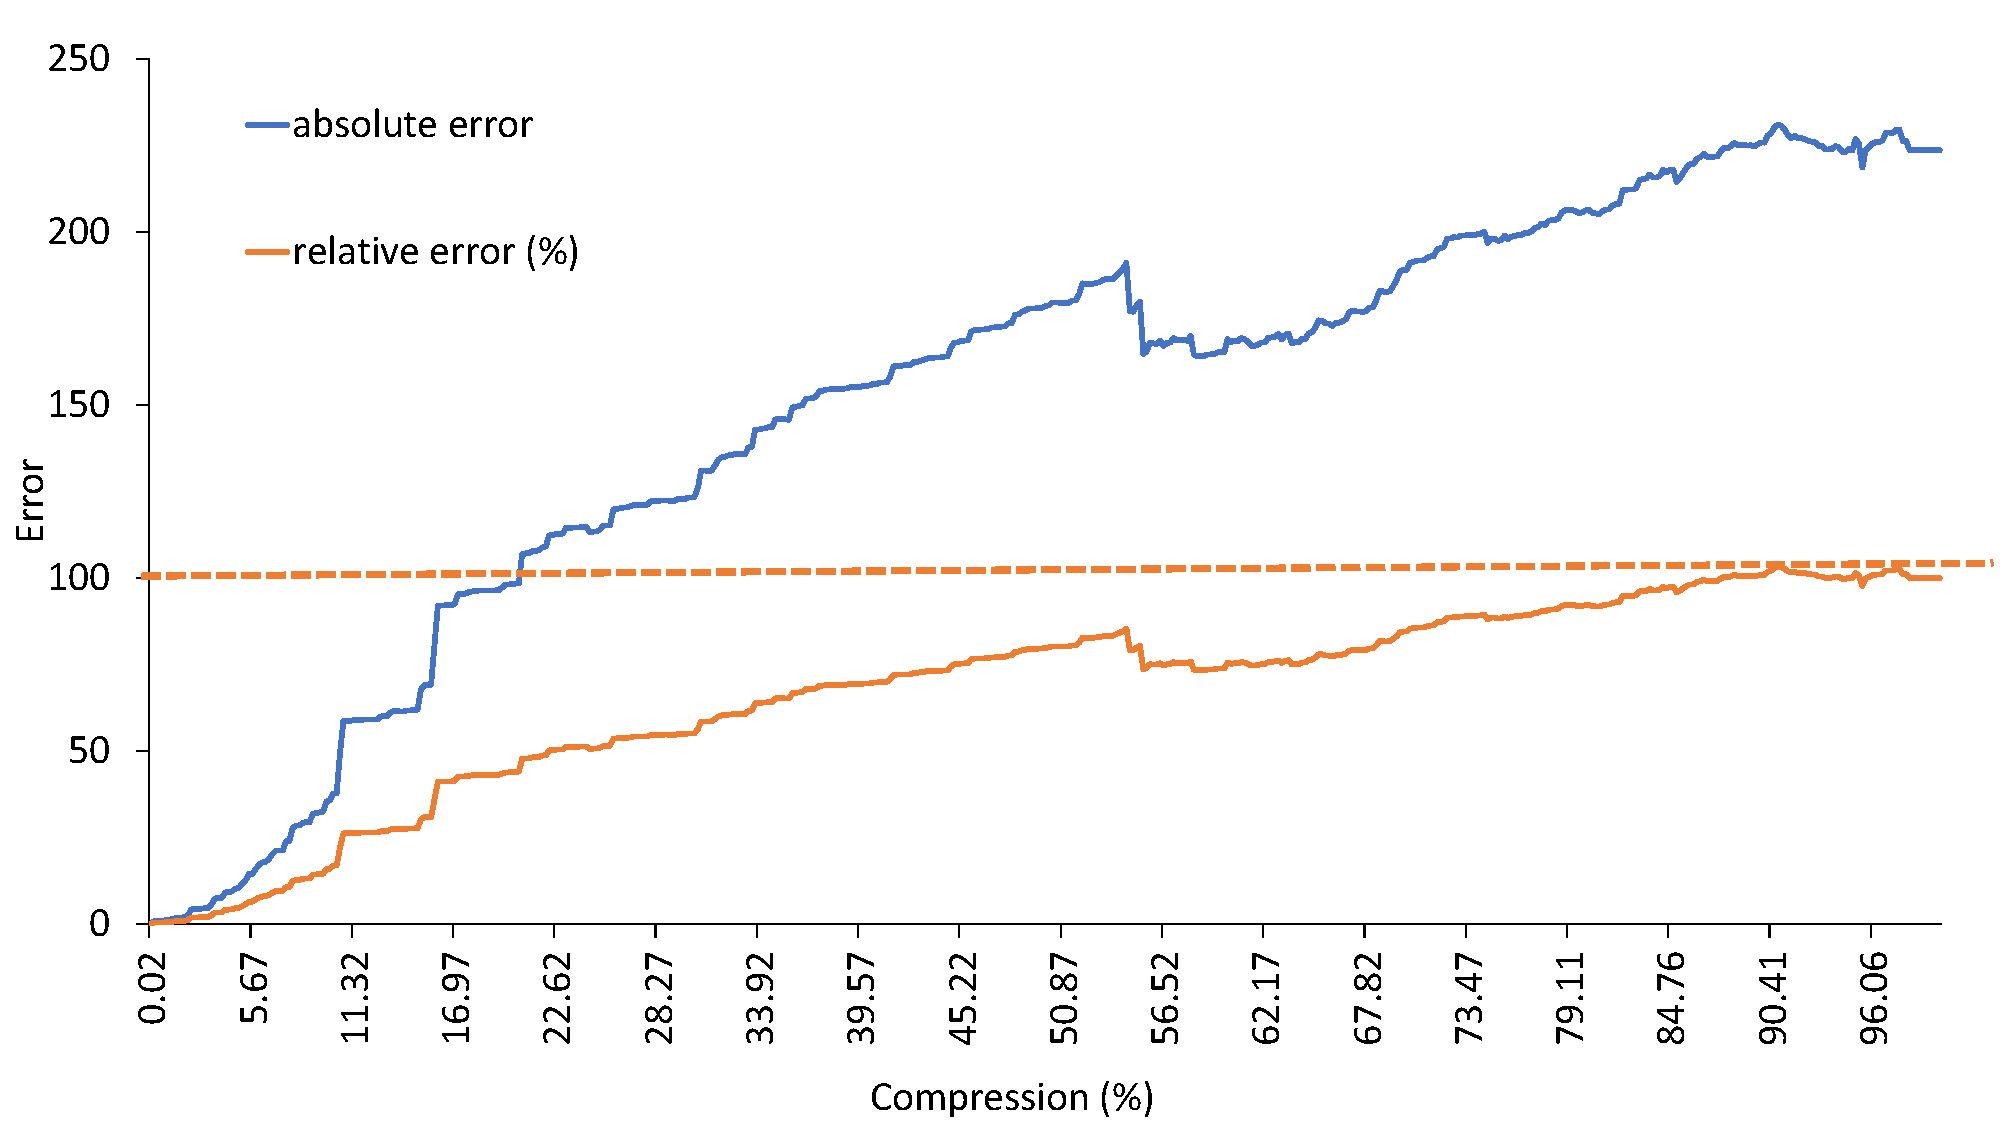
\includegraphics[width=\linewidth]{conv2DrelativeErrorGraph.pdf} %width=\linewidth]
  \caption{{\it A comparison of the relative (in \%) and absolute errors between 2D convolution from PyTorch (which is our gold standard with high numeric accuracy) and a fine-grained top compression method for a CIFAR-10 image and a 5x5 filter (with 3 channels).
}}
  \label{fig:compareErrorsFFT2Dconv-supplement}
\end{figure}

We plot in Figure\ref{fig:compareErrorsFFT2Dconv-supplement} fine-grained compression using the top method (the coefficients with lowest values are zeroed-out first). For a given image, we compute its FFT and its spectrum. For a specified number k of elements to be zeroed-out, we find the k smallest elements in the spectrum and zero-out the corresponding elements in the in the image. The same procedure is applied to the filter. Then we compute the 2D convolution between the compressed filter and the image. We do not remove the elements from the tensors (the sizes of the tensors remain the same, only the smallest coefficients are zeroed-out). The plots of the errors for a given compression (rate of zeroed-out coefficients) are relatively smooth. This shows that our method to discard coefficients and decrease the tensor size is rather coarse-grained and especially for the first step, we remove many elements.

We have an input image from CIFAR-10 with dimensions (3x32x32) which is FFT-ed (with required padding) to tensor of size (3x59x30). We plot the graph in 10 element zero-out step, i.e. first we zero-out 10 elements, then 20, and so on until we reach 5310 total elements in the FFT-ed tensors). The compression ratio is computed as the number of zeroed-out elements to the total number of elements in FFT-ed tensor. There are some dips in the graph, this might be because the zeroed-out value is closer to the expected value than the one computed with imprecise inputs. With this fine-grained approach, after we zero-out a single smallest coefficients (in both filter and image), the relative error from the convolution operation is only 0.001\%. For the compression ratio of about 6.61\%, we observe the relative error of about 8.41\%. In the previous result, we used the lead method and after discarding about 6.6\% of coefficients, the relative error was 22.07\%. For the lead method, we were discarding the whole rows and columns across all channels. For the fine-grained method, we select the smallest elements within the whole tensor.

\subsection{Time-series data}
\begin{figure}[t]
  %
\includegraphics[width=\linewidth]{figures/conv2D-cifar10-leNet-test-accuracy.pdf} %width=\linewidth]
  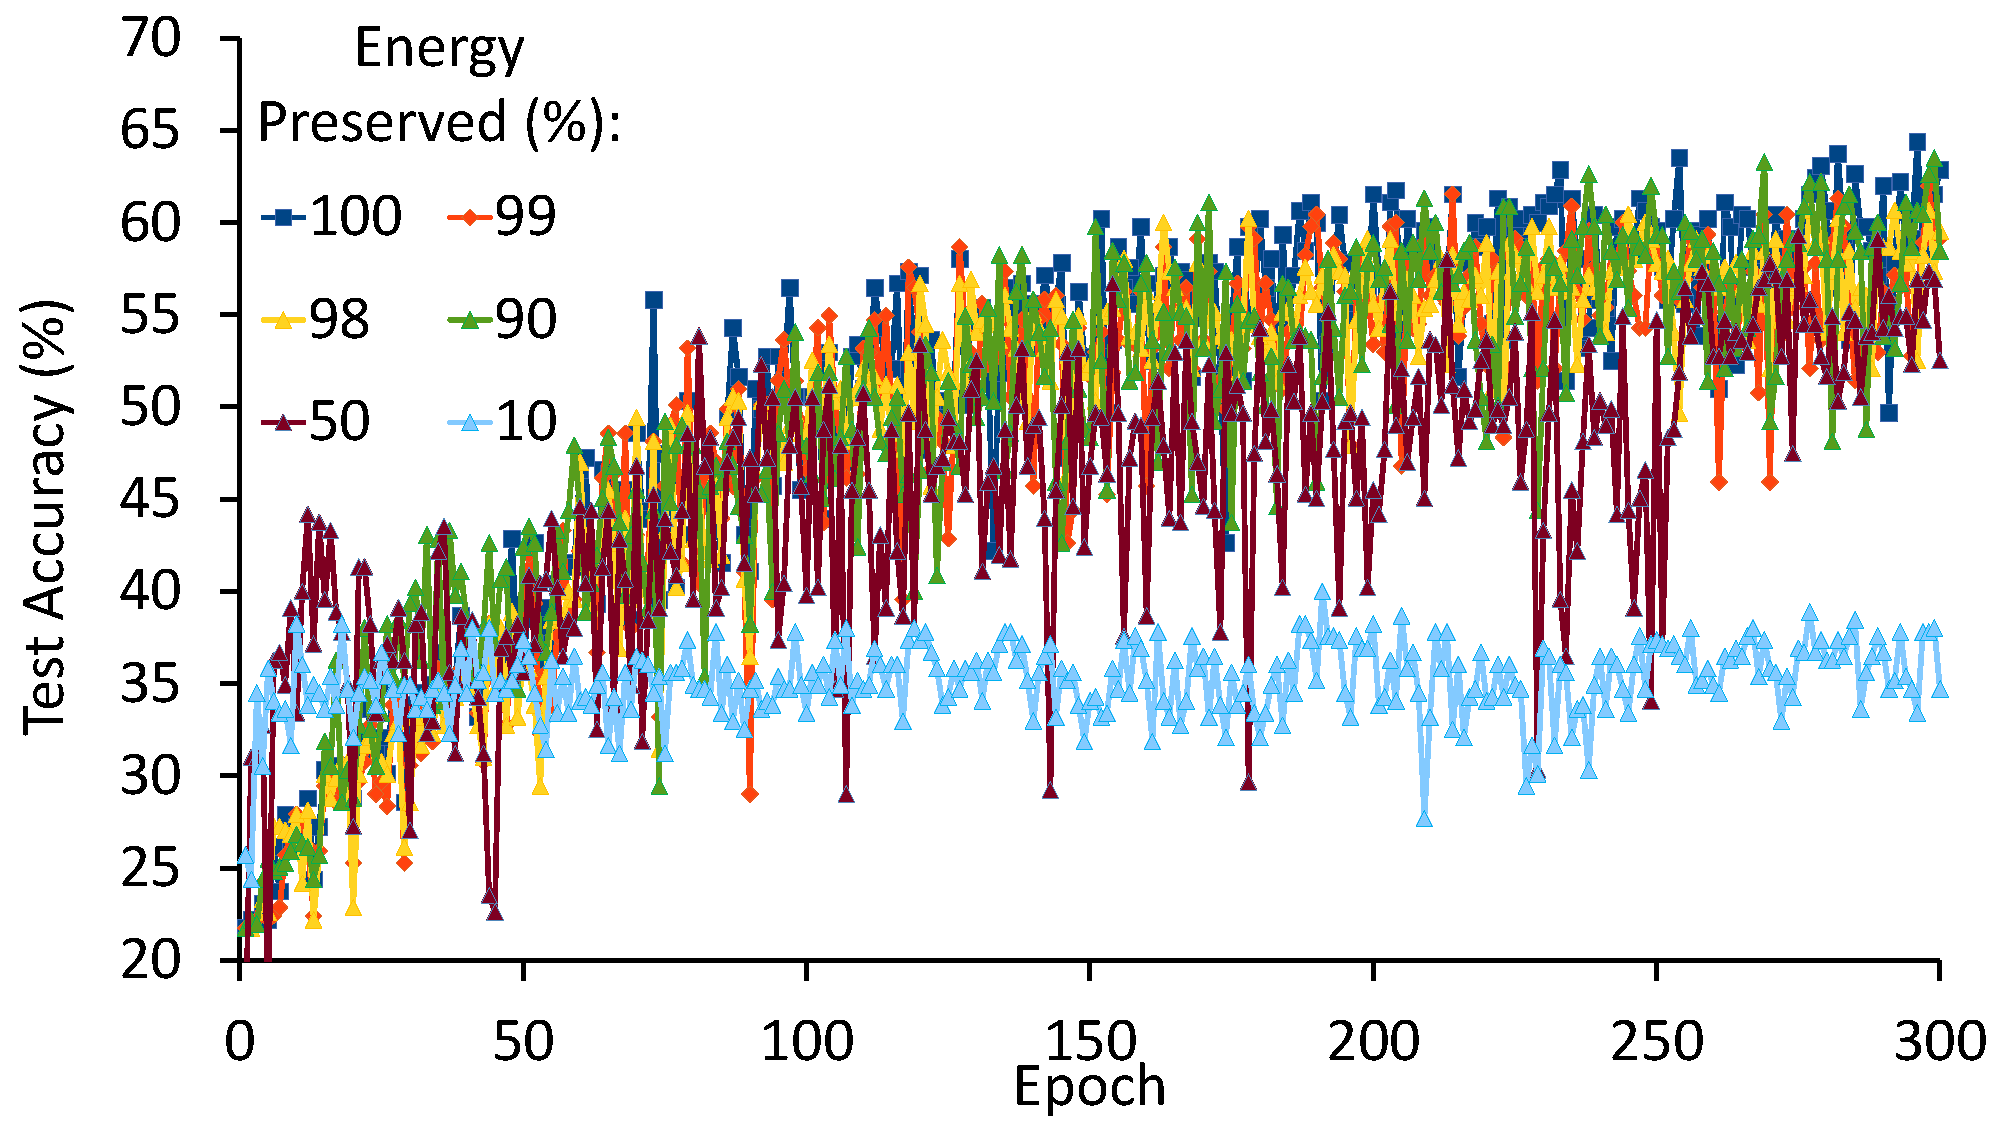
\includegraphics[width=\linewidth]{AccuracyConv1D50wordsFCN.pdf} %width=\linewidth]
  \caption{{\it Test accuracy on a 3 layer FCN architecture for 50 words time-series dataset from the UCR archive.}}
  \label{fig:AccuracyConv1D50wordsFCN}
\end{figure}

% \begin{table*}
% \centering
% \ra{1.3}
% \begin{tabular}{@{}lll@{}}
% \toprule
% \multicolumn{1}{|p{3cm}|}{\centering Energy\\ preserved (\%)} & &
% \midrule
% 100 & 118 & 64.40 \\
% \bottomrule
% \end{tabular}
% \caption{Maximum test accuracy for a given GPU memory usage and corresponding energy preserved in the signal (we compute the memory usage by counting the size of all tensors used).
% }
% \end{table*}

\begin{figure}[t]
  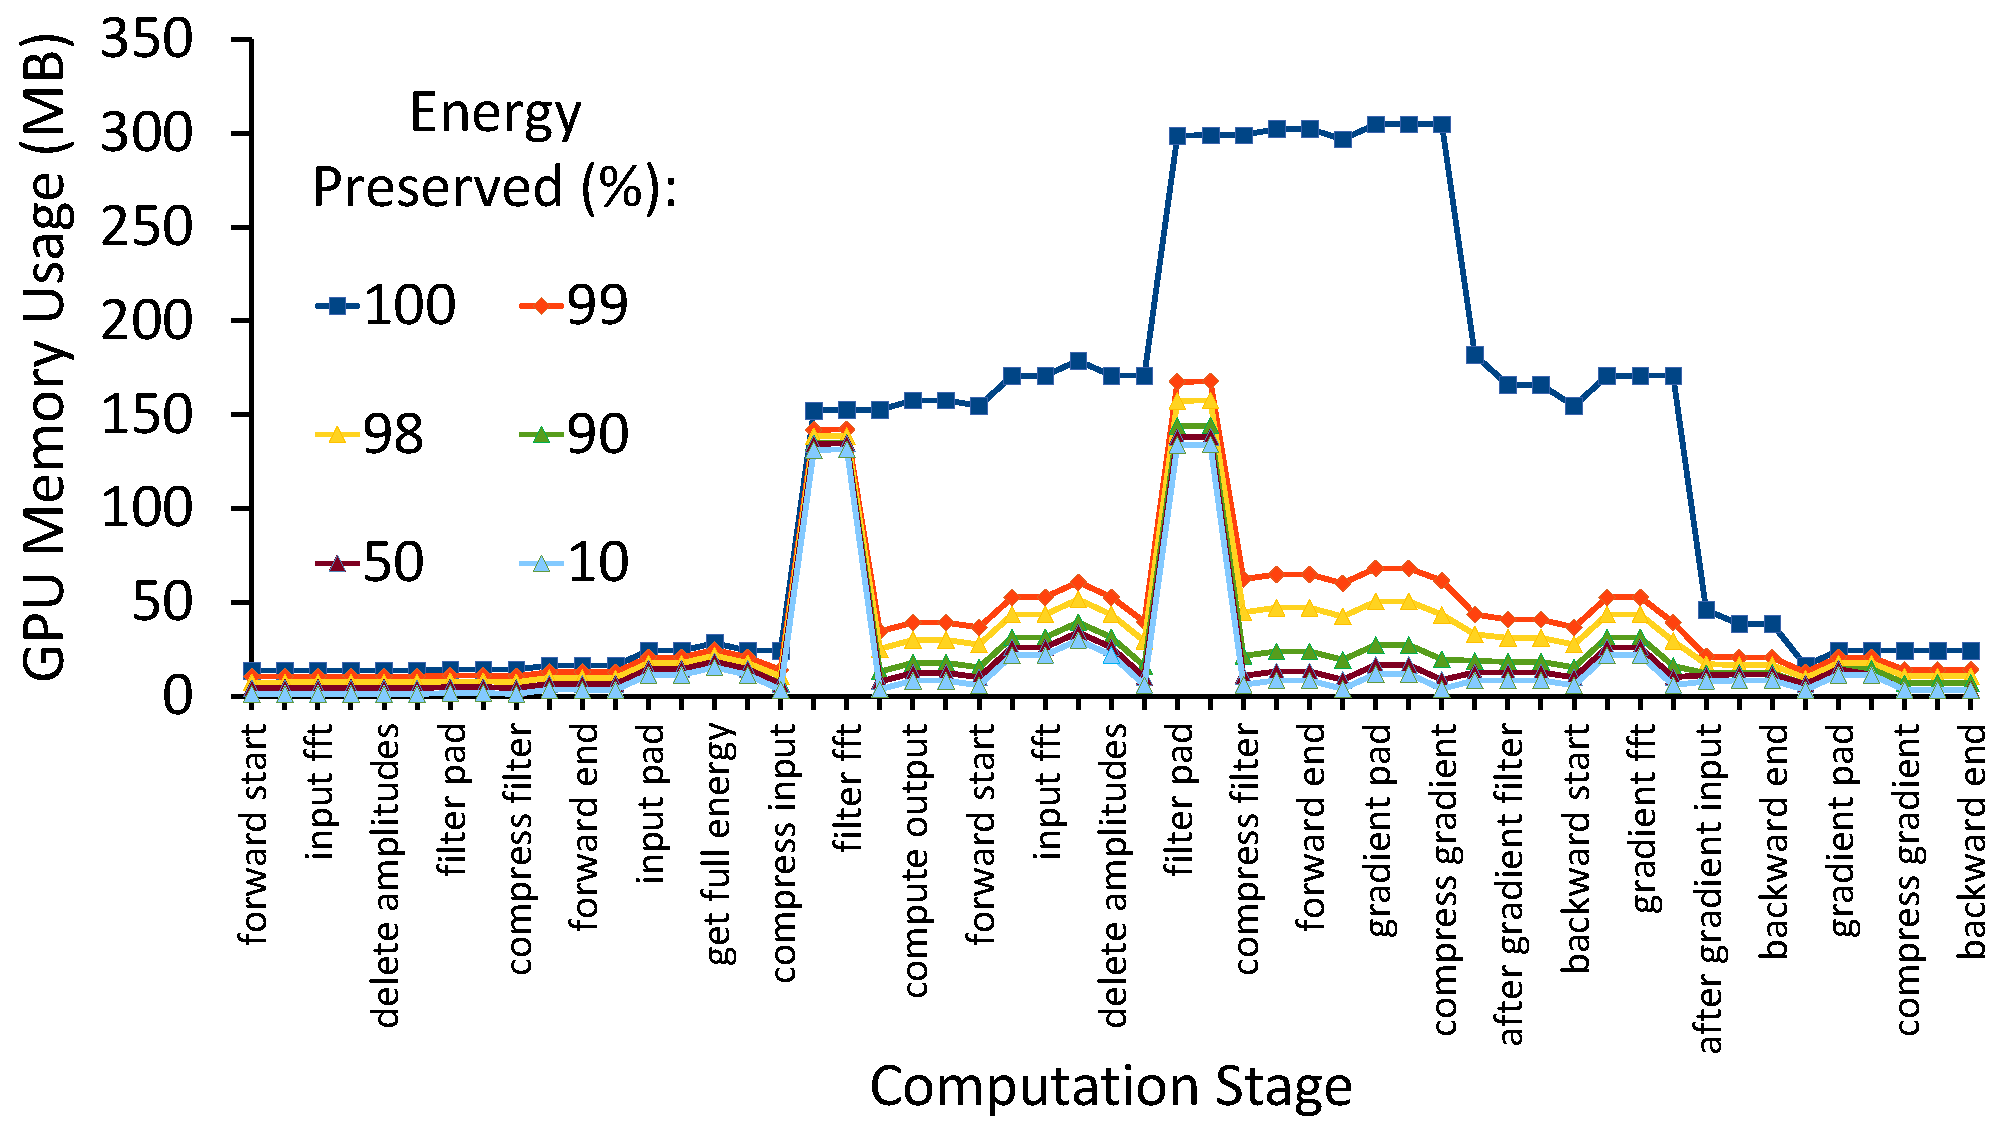
\includegraphics[width=\linewidth]{GPUmemUsage.pdf} %width=\linewidth]
  \caption{{\it GPU memory usage (in MB) during training for a single forward and backward pass through the FCN network using 50 words dataset.}}
  \label{fig:GPUmemUsageConv1D50wordsFCN}
\end{figure}

We show the accuracy loss of less than 1\% for 4X less average GPU memory utilization (Figures:~\ref{fig:AccuracyConv1D50wordsFCN} and~\ref{fig:GPUmemUsageConv1D50wordsFCN}) when training FCN model on 50 words time-series dataset from the UCR archive. 
\begin{figure}[t]
  %
\includegraphics[width=\linewidth]{figures/conv2D-cifar10-leNet-test-accuracy.pdf} %width=\linewidth]
  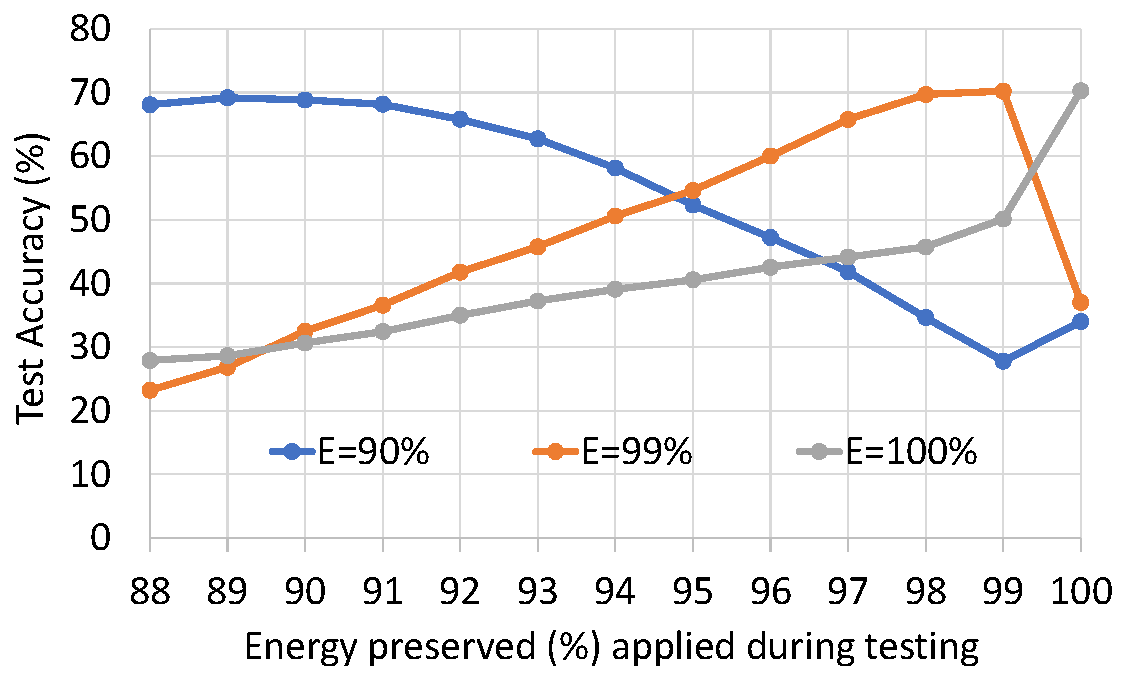
\includegraphics[width=\linewidth]{compression_levels_for_testing_training.pdf} %width=\linewidth]
  \caption{{\it We train three models on the time-series dataset \textit{uWaveGestureLibrary\_Z}. The preserved energy during training for each of the models is 90\%, 99\% and 100\% (denoted as E=X\% in the legend of the graph). Next, we test each model with energy preserved levels ranging from 88\% to 100\%. We observe that the highest accuracy during testing is for the same energy preserved level as the one used for training and the accuracy degrades smoothly for higher or lower levels of energy preserved.}}
  \label{fig:compressionLeveslTrainTest}
\end{figure}

In Figure~\ref{fig:compressionLeveslTrainTest} we show the training compression vs. inference compression for time-series data. This time we change the compression method from static to the energy based, however, the trend remains the same. The highest test accuracy is achieved by the model with the same energy preserved during training and testing.

% \begin{table}[t]
% \caption{Max. and Avg. memory usage with corresponding compression ratio for each layer. We compute the compression ratio as: $\frac{\text{input size}}{\text{FFT compressed size}}$. For example, for the first convolutional layer (conv1), which has 270 input values, there are 1024 values in the frequency domain, thus for 100\% compression ratio we obtain:  $\frac{270}{1024}=0.26$, for 99\% compression ratio: $\frac{270}{181}=1.49$, where 181 is the length of the compressed signal.}
% \label{tab:mem-usage-each-conv-layer}
% \vskip 0.15in
% \begin{center}
% \begin{small}
% \begin{sc}
% \begin{tabular}{cccccc}
% \toprule
% \multicolumn{2}{c}{Memory usage (MB)} & \phantom{a} & \multicolumn{3}{c}{Compression ratio}\\
% \cmidrule{1-2} \cmidrule{4-6}
% Max. & Avg. && conv1 & conv2 & conv3 \\
% \midrule
% 305 & 118 & & 0.26 & 0.27 & 0.27 \\ 
% 168 & 41 & & 1.49 & 2.21 & 2.76 \\
% 158 & 34 & & 1.99 & 2.96 & 3.71 \\
% 144 & 25 & & 4.23 & 6.62 & 9.40 \\
% 138 & 21 & & 11.29 & 27.80 & 47.00 \\
% 134 & 17 & & 33.88 & 139.00 & 141.00 \\
% \bottomrule
% \end{tabular}
% \end{sc}
% \end{small}
% \end{center}
% \vskip -0.1in
% \end{table}

% \subsection{Shapes of filters, activations and gradients in the frequency domain.}
% We chose dataset 50 words from the UCR archive, the FCN network with 3 convolution layers (each followed by a ReLU and batch normalization) and preserve 90\% of the energy in the activations.

%  Neural networks are biased towards low frequency functions, thus they tend to better approximate the smooth functions or natural images with small amount of noise. The question is if our lead compression method can be applied to the filters. We observe a transformation of the filter (in the last layer of FCN) from a random shape to a slope starting high for low frequencies and going down with increasing frequencies, which suggests that the network learned the low frequency values of the filters as constrained by our compression.

% The representation of the input signal in the frequency domain shows the highest (signal) values for the low frequency values. The most important outcome is that the data inputs (activations) after the convolution operation retain their shape and the (signal) highest values are preserved for the low frequency values. This is because when we consider the convolution operation in the frequency domain, the element-wise multiplication between the input that has very small or zero values for all frequencies but the low ones, hence irrespective of the filter shape, the high signal values should remain only for the low frequency values after the convolution. 
% We also plot the spectra of the flowing back gradients in the time and spectral domains. The gradients are generated for the output. The output from the convolution operation preserves the property that the highest values of the signal remain in the regime of low frequencies, thus also the gradients follow the same pattern. The only problematic part of the analysis is that the filters are relatively small and they do have high signal values even for the high frequencies (that usually represent noise for natural images), for example, for the 1st layer of FCN. Our method to deal with the problematic behavior would be to try to initialize the filters in the frequency domain with higher values for lower frequency and manage the filters only in the frequency domain, since the transformations of the filter back and forth between time and spectral domain are unnecessary.

% Example of the spectral representations of a gradient (for the output of the convolution operation):

\subsection{Robustness to Adversarial Examples}
We present the most relevant adversarial methods that were executed using the foolbox library. Our method is robust to decision-based attacks (GaussianBlur, Additive Uniform or Gaussian Noise) but not to the gradient-based (white-box and adaptive) attacks (e.g., Carlini \& Wagner or FGSM) since we return proper gradients in the band-limited convolutions. If an adversary is not aware of our band-limiting defense, then we can recover the correct label for many of the adversarial examples by applying the FFT compression to the input images.

\begin{figure}[ht!]
\centering
  %
\includegraphics[width=\linewidth]{figures/conv2D-cifar10-leNet-test-accuracy.pdf} %width=\linewidth]
  %\includegraphics[width=0.8\linewidth]{figures/gaussian-noise/gaussian_noise.pdf}
  %\includegraphics[width=\linewidth]{figures/gaussian-noise/gaussian_noise.pdf}
  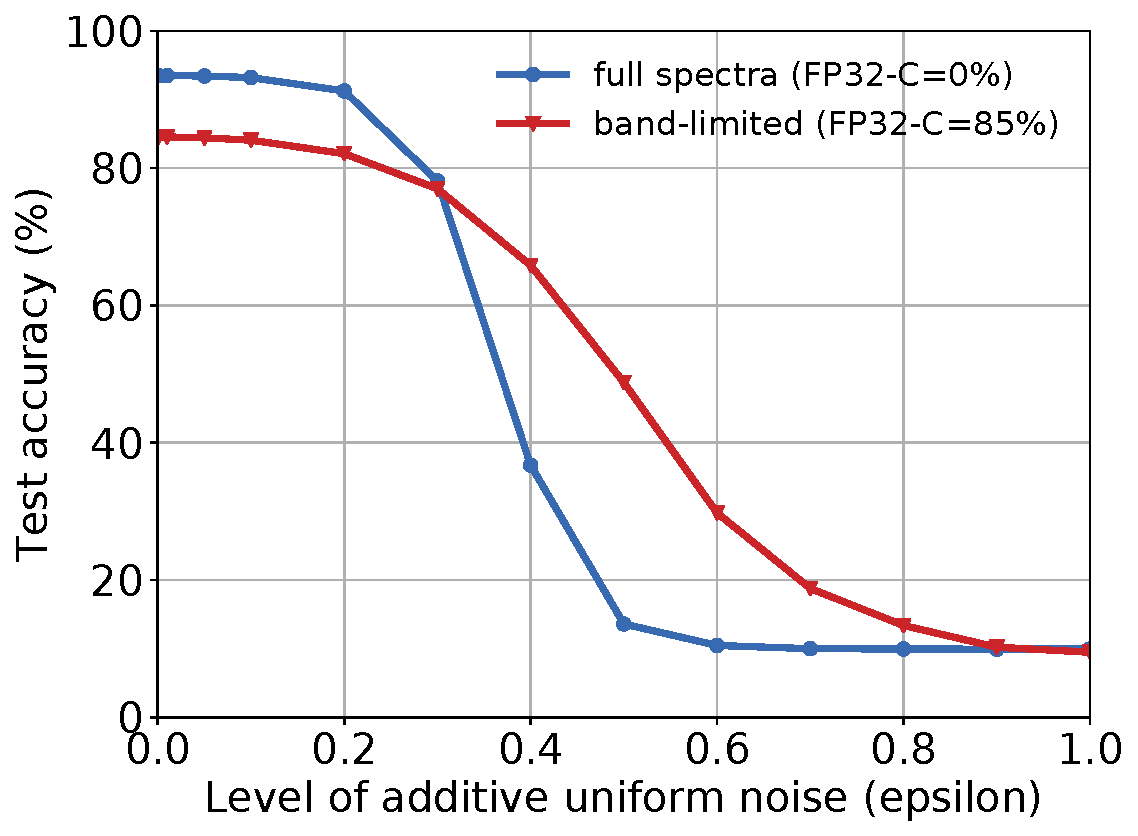
\includegraphics[width=0.6\linewidth]{uniform_noise-font.pdf}%width=\linewidth]
  \caption{{\it Input test images are perturbed with additive uniform noise, where the epsilon parameter is changed from 0 to 1. The more band-limited model, the more robust it is to the introduced noise. We use ResNet-18 models trained on CIFAR-10.}}
  \label{fig:uniform-noise}
\end{figure}

